\documentclass[12pt,a4paper]{article}
\usepackage{amsmath,amssymb,amsthm}
%\usepackage[semicolon,sort]{natbib}



\newtheorem{hyp}{Hypothesis}
\newtheorem{res}{Result}

\title{
Group-Based Upstream Reciprocity.%
\thanks{
This research was supported by the ISRAEL SCIENCE FOUNDATION (grant No. 214/13)
}}
\author{David Hugh-Jones\thanks{School of Economics, University of East Anglia. E-mail: d.hugh-jones@uea.ac.uk.} \and Itay Ron\thanks{E-mail: itayron@gmail.com} \and Ro'i Zultan\thanks{Department of Economics, Ben-Gurion University. E-mail: zultan@bgu.ac.il.}}

\date{\sffamily \small This version: \today.} % \\ \textbf{Preliminary version, please do not distribute.}}

\def\figwidth{\textwidth}

\begin{document}
\maketitle

\begin{abstract}
% original version was too timid and spent too little time on our own contribution. Suggest:
Cycles of intergroup revenge appear in large scale conflicts. We experimentally test the hypothesis that humans
practice group-based reciprocity: if someone harms or helps them,
they harm or help other members of that person's group. Subjects played a trust game, then allocated money between other people.
Senders whose partners returned more in the trust game gave more to that partner's group members. The effect was about 60 per cent
of the size of the direct reciprocity effect. Receivers' allocations to group members did not depend on their partner's play, suggesting
that group reciprocity was only triggered when the partner's intentions were unequivocal.

\section{Introduction}

The evolution of cooperation poses a puzzle to evolutionary and social scientists. Cooperation---by which individuals forgo personal benefits to aid others---is a hallmark of human uniqueness. On the other hand, there is a direct evolutionary pressure selecting against cooperators in favour of free riders. One mechanism that may underlie the evolution of cooperation is reciprocity \citet{nowak2006five,nowak2012evolving,}. Direct reciprocity increases the fitness of cooperators, as helping another individual leads to that individual reciprocating the help. In indirect reciprocity, individuals help or harm other people than those who have helped them.

Evidence suggests that human social behaviour, including cooperation and reciprocity, is bounded by social groups \citep*{tajfel1979integrative,balliet2014ingroup,DeDreu2014}. Humans cooperate more with, and reciprocate more towards members of their group \citep*{chen2009group,chen2011potential}; and they punish norm violators more who harm a member of their own group \citep*{bernhard2006group,bernhard2006parochial}.

% think we shd cite Yamagishi 1985 above also.

Group identities may also affect reciprocity in another way: humans take revenge on outgroups as well as on individuals. Cycles of intergroup revenge appear widespread in human conflict \citep*{}. Surprisingly little work has examined this motivation. Existing experiments on `vicarious retribution' are suggestive but lack material incentives or correct control. \citep*{XXX}. We ran a laboratory experiment to test for the existence of group-based reciprocity and compare its strength to direct, individual-level reciprocity.

% the last 2 sentences should be a footnote maybe

% what do we cite? Horowitz 1985 and 2001; maybe Chagnon 1988; maybe WB 2011 for why conflict is so bad. Maybe Shayo and Zussman 2011, 2012. Psychological cites are Yzerbyt etc.


Indirect reciprocity comes in two flavours; \emph{downstream} reciprocity follows the principle of `do unto thy neighbour as they have done to others', whereas \emph{upstream} reciprocity follows the principle of `do unto thy neighbour as others have done unto you'. In this paper we study upstream indirect reciprocity \citep*{nowak2005evolution,nowak2007upstream,boyd1989evolution}. Compared to downstream reciprocity, upstream reciprocity is simpler to implement, as it does not require tracking individual reputations, but is more difficult to understand from an evolutionary point of view \citep*{nowak2005evolution,boyd1989evolution}. Nonetheless, upstream reciprocity can co-evolve with direct or spatial reciprocity \citep*{nowak2007upstream}. Laboratory experiments provide positive evidence for upstream reciprocity, as individuals are more generous to others if a third party was generous to them \citep*{dufwenberg2001direct,guth2001trust,greiner2005indirect}, and the mere possibility of being harmed by a third party reduces cooperation in a social dilemma \citep*{weisel2016social}.


The notion we introduce here, of group-based upstream reciprocity, or \emph{group reciprocity}, generalizes this observation by arguing that people are also sensitive to the social identity of \emph{others}, essentially differentiating between different types of `others'. Thus, if group-based downstream reciprocity \citep*{bernhard2006group,bernhard2006parochial} follows the dictate `do unto others as they have done to members of \emph{my} tribe', group-based upstream reciprocity follows the dictate `do unto others as members of \emph{their} tribe have done to me' (Figure~\ref{fig:illustration}).

We ran a laboratory experiment to test the hypothesis that people reciprocate in groups. After an initial group-formation stage, participants interacted in two strategic stages. The first stage represented the upstream interaction, in which the individual could be helped by another person. We implemented this as a Trust Game \citep*[TG,][]{berg1995trust}, in which the Sender~(S) receives~150 money-equivalent tokens, and chooses how many of them to send to the Responder~(R). The amount sent is multiplied by a factor of~3, so that R receives between 0~and~450 tokens, of which he can send any number back to~S. The TG enables us to model two types of interactions. Whereas~R is clearly kind when returning money (and nasty when exploiting a generous proposer by keeping the received amount), S's intentions are equivocal. Sending money can be driven by selfish expectations of reciprocity, while not sending can be driven by cautiousness. Thus,~R experiences kind or nasty \emph{actions}, while~S experiences kind or nasty actions and \emph{intentions}.

% upstream, not downstream, right:?
The second stage represented the reciprocal action, in which the individual could help others. We implemented this interaction as an allocation game (AG), in which an allocator allocates a fixed amount between two recipients. In direct reciprocity (DR) rounds, the recipients included the TG partner; in group reciprocity (GR) rounds, a member of the TG partner's group; and in in-group favouritism (IF) rounds, a member of the allocator's group. The other recipient was always a member of a third, neutral, group. Baseline (B) rounds included two neutral recipients, to test whether the TG experience lead allocators to discriminate in absence of any reciprocal or group motivations.

The allocation decisions revealed that reciprocating intentions generalizes to groups. The effect of group-based upstream reciprocity was approximately 63\% of that of direct reciprocity. Although we found strong evidence for direct reciprocity of actions, this did not generalize to the group level. Allocations favoured in-group members, indicating that our group manipulation was successful.

\begin{figure}
	\begin{center}
        \begin{subfigure}[b]{0.4\textwidth}
		  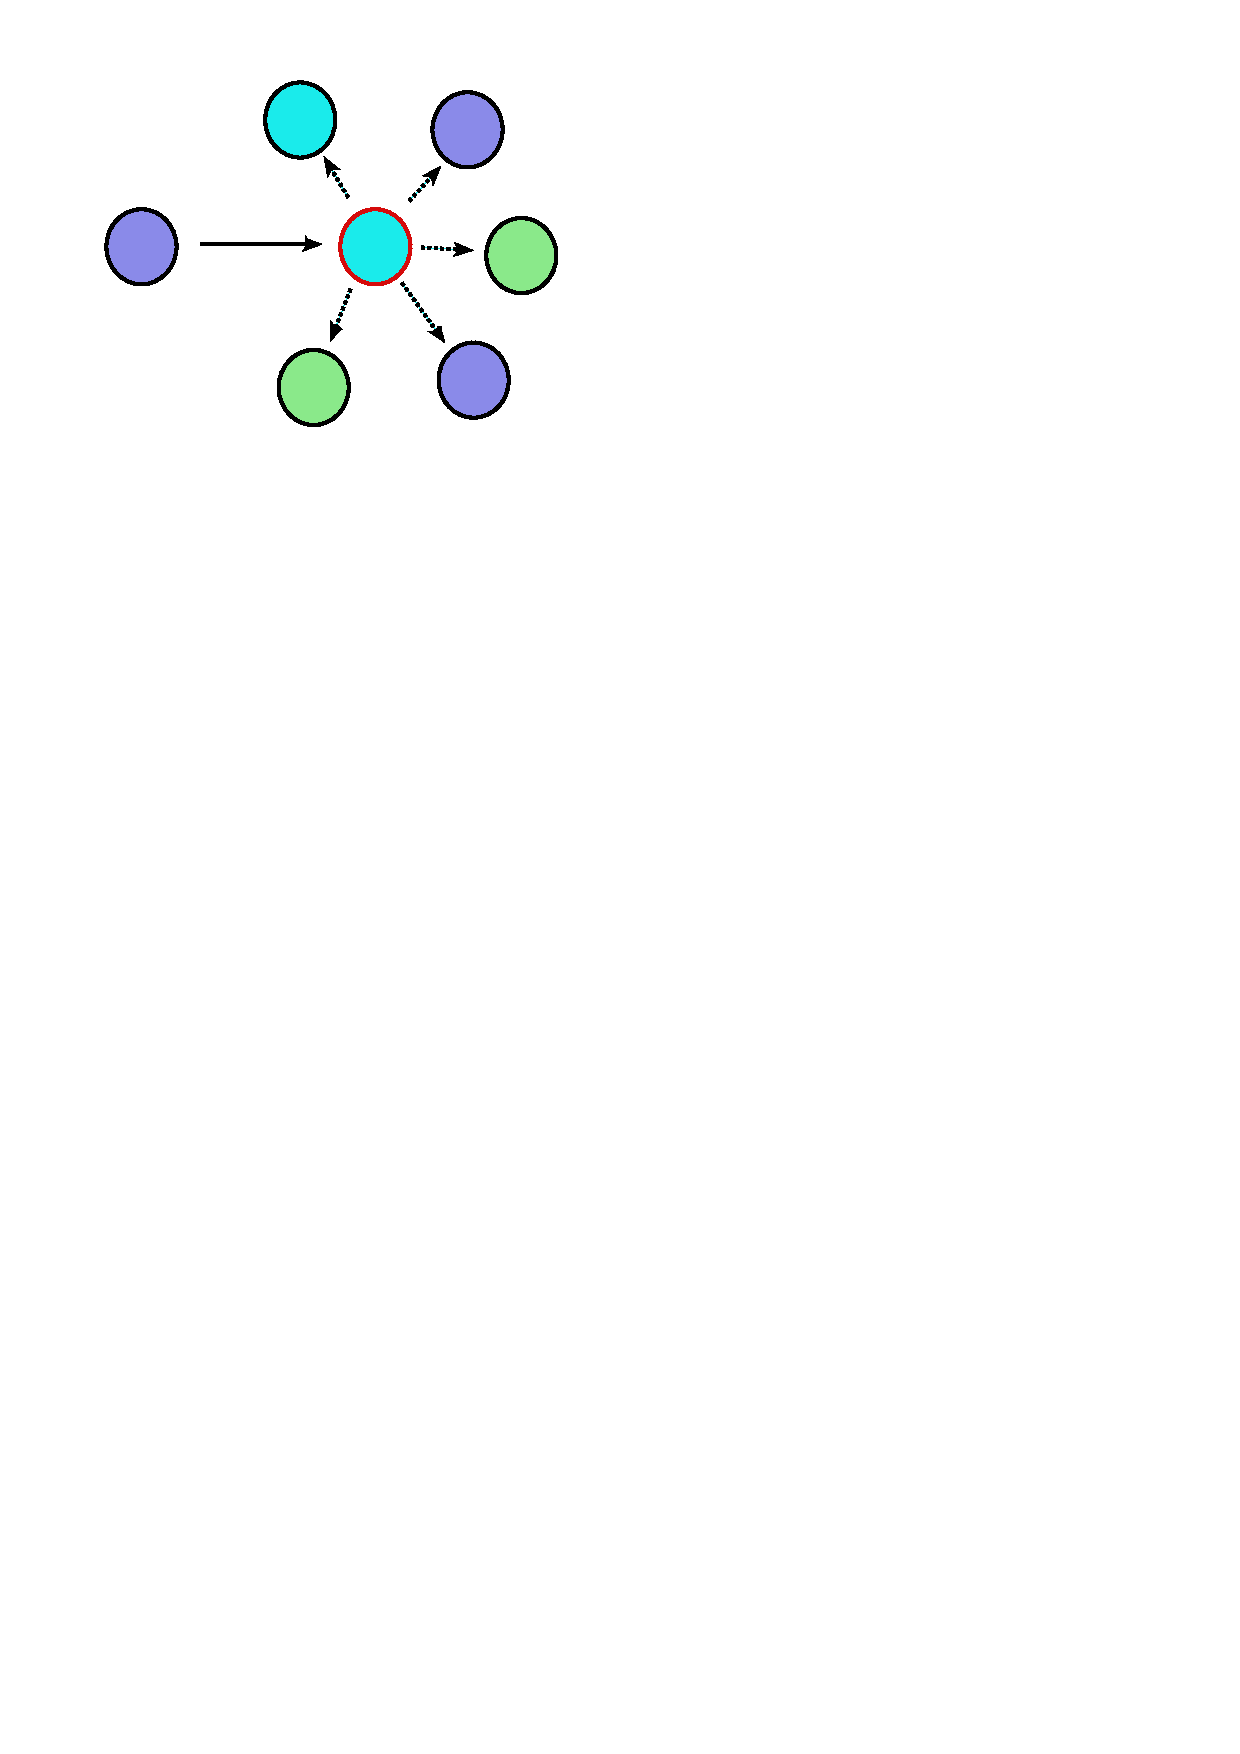
\includegraphics[width=\textwidth]{upstream.pdf}
            \caption{}\label{upstream}
        \end{subfigure}
        \qquad
        \begin{subfigure}[b]{0.4\textwidth}
		  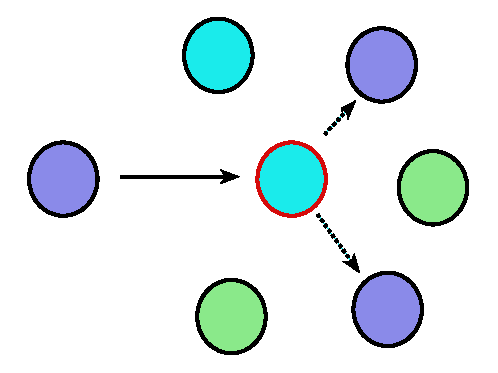
\includegraphics[width=\textwidth]{group.pdf}
            \caption{}\label{group}
        \end{subfigure}
        \caption{Upstream reciprocity. (\textit{a}) Someone who was helped or harmed becomes equally more likely to help or harm new partners. (\textit{b}) Upstream reciprocity is particularly directed at new partners that belong to the same group as the initial partner.}
        \label{fig:illustration}
	\end{center}
\end{figure}

\section{Method}
\label{sec:design}

Each session consisted of~24 participants, who were randomly allocated to six groups of four. To distinguish from the groups in which participants interacted throughout the different stages of the experiment, we refer to the identity-relevant initial group as a \emph{Team}.
Each participant was identified throughout the experiment by team colour and individual number (1--4) within the team. At the beginning of the experiment, we informed participants that the experiment has five distinct stages. In each stage, new groups are formed, and it is possible (though not necessary) that two participants will be in the same group in two different stages. The specific instructions for each stage were distirbuted and read aloud at the beginning of the stage. The five stage were a group formation stage, the TG stage, the AG stage, a social value orientation elicitation \citep*{murphy2011measuring} stage and a collectivism scale measurement \citep*[adapted from the horizontal collectivism scale in][]{Singelis1995horizontal}.

Following \citet*{chen2009group}, we created group identity in the first stage by allowing participants to consult each other using anonymous chat when solving a simple task. Participants solved five Raven matrices (see supplementary material). Each matrix was presented on screen for 120~seconds, during which each participant could both send written messages to the team and update her own answer. The final answer submitted at the end of the 120~seconds determined payoffs, with 10~tokens paid for each ocrrect answer. To further boost group identity through a common goal, an additional bonus of 5~tokens was earned if all four team members answered correctly.

Next, participants were rematched into pairs to play the one-shot TG. To facilitate understanding, participants played five practice rounds, in which they entered decisions both as~S and as~R. In the actual interaction, participants could see their TG partner's team colour and individual number. The kindness of the Sender was measured as the share of the endowment sent, and of the Responder as the share of the received amount sent back. Responder's kindness was not defined for six (out of 96) responders whose partner did not send any money.

The third stage consisted of six rounds. In each round, participants interacted in a group of three, identified by team colour and number. The allocation game was implemented as a random dictator game as follows. Each player in the group of three received 100~tokens to allocate within the group. The allocator received 30~tokens, and could freely allocate the remaining 70~tokens between the other two players. Previous research found that people do not harm, but refrain from helping negatively perceived out-groups. Accordingly, we set the parameters of the game such that, compared to the reference point of the allocator's own share, an equal division benefits both other players. The matching scheme ensured that over the six rounds, each participant was in the same group of three exactly once with a member of her own team (treatment IG), once with her TG partner (Treatment DR), and twice with other members of the TG partner's team (treatment GR). The remaining two rounds served as the baseline (B) treatment. For example. Note that the matching is not independent. For example, if one player is in treatment DR, than the other two are in treatments Dr and either B or GR. No feedback was provided between rounds.
The payoffs for this stage were determined by one randomly chosen round of the six rounds, and the allocator decision of one randomly chosen player in each group.

The fourth stage implemented the slider measure \citep*{murphy2011measuring,crosetto2012flexible}, in which participants choose nine allocations between themselves and another person. For consistency with the previous stages, the team identity of the partner was known. To keep the decision independent of previous experience with the different teams, we matched participants within teams. Consistent with the notion of humans as parochial altruists, we believe that such in-group allocations best reflect social preferences.
Payoffs were determined by one randomly chosen decision of the nine decisions made by one randomly chosen player in each dyad.
The decisions yielded for each participant a social orientation angle, with~$0^\circ$ corresponding to selfishness, $45^\circ$ to pure altruism, and negative angles to spitefulness.

After the fifth and final stage of non-strategic and non-incentivised collectivism measurement, participants learned of their cumulative payoff in tokens, and final payment in New Israeli Shekels.  One hundred and ninety two participants, recruited using ORSEE \citep*{greiner2015subject} participated in eight sessions conducted between June 2014 and January 2015. Due to software malfunction in one session, the data from the AG sixth round were not saved.
The experiment was programmed in z-Tree \citep*{Fischbacher2007}. The average payment was 72~NIS (approximately \$18) for a duration of 70~minutes.

\section{Results}
\label{sec:results}

We report results on allocations, discrimination between recipients, and direct and group reciprocity. All reported statistical tests are based on mixed-effects regressions with robust standard errors clustered on subjects. See the supplementary material for the full specification and results.

Figure~\ref{fig:allocations} presents the mean allocations. Participants gave significantly more to members of their own team at the expense of the neutral recipient ($\beta = 6.76, p<0.001$ for senders, $\beta = 4.25, p<0.005$), establishing that our group formation manipulation was successful in inducing group identity and triggering in-group favouritism. Allocations to the TG~partner and his team mates were not significantly different to the baseline~35 ($p>0.440$ for all comparisons). Nonetheless, allocators discriminated significantly more than in the baseline both when interacting with their TG partner ($\beta = 19.18, p<0.001$) and with his team mates ($\beta = 4.04, p<0.001$. The interaction of the identity of the recipient and the allocator's TG role (sender or reciever) was not significant ($\chi^2 = 1.42, p = 0.700$).

\begin{figure}
\caption{
Allocations by TG role and experimental condition with~95\% confidence intervals based on subject-level averages. Allocations to the TG partner and her team mates are not significantly different, on average, to the baseline allocation of~35 tokens. Allocators give significantly more to their own team mates. Allocations are at the expense of a neutral-team recipient.
}
\label{fig:allocations}
\begin{center}
	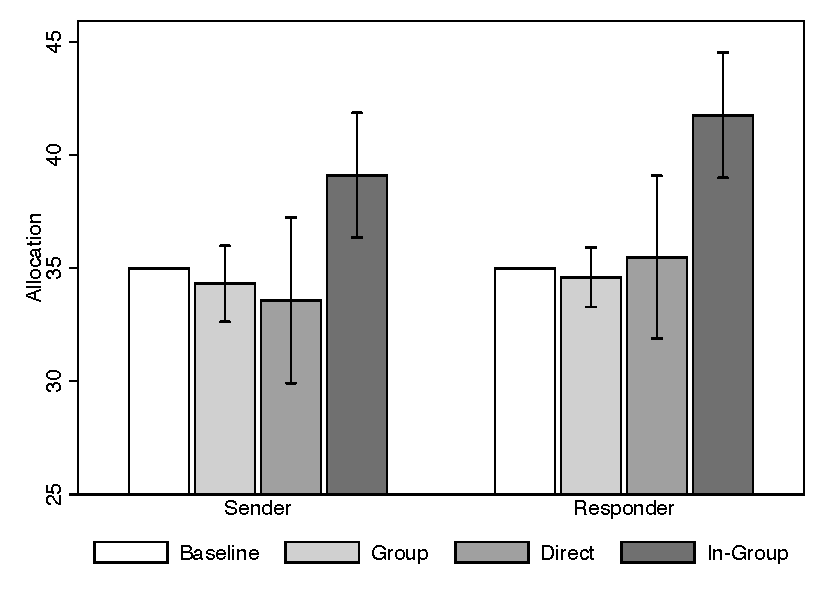
\includegraphics[width=\figwidth]{Allocations.pdf}
\end{center}
\end{figure}


\begin{figure}
\caption{
Discrimination between the two recipients by TG role and experimental condition with~95\% confidence intervals based on subject-level averages. Allocators discriminate more when one of the two recipients is their own team mate, their TG partner, or their TG partner's team mate.
}
\label{fig:discrimination}
\begin{center}
	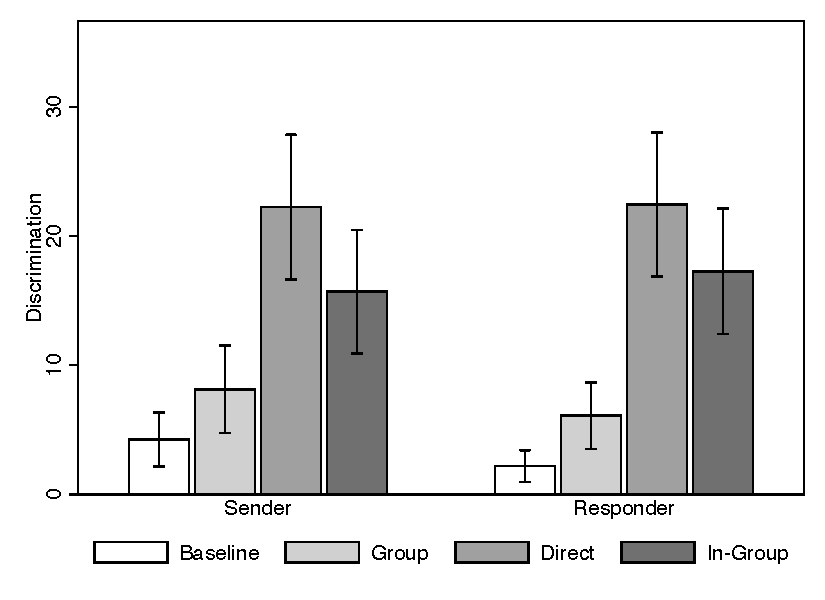
\includegraphics[width=\figwidth]{Discrimination.pdf}
\end{center}
\end{figure}

\subsection*{Direct and group reciprocity}
\label{sec:reciprocity}

Figure~\ref{fig:reciprocity} presents the allocations made in the DR and GR conditions separated by the whether the kindness of the action of the TG partner was below the median or not. The median kindness of the senders was~$\frac{1}{2}$ (median transfer of~75 out of~150 tokens). The median kindness of the responders was~$\frac{1}{3}$ (median share returned matches the amount sent). The figure reveals strong direct reciprocity. Senders allocate less than the baseline~35 tokens to responders who failed to at least compensate the sender for the amount sent. Responders both allocate more than~35 tokens to senders who sent at least half their endowment, and less to those who sent less.
These observations are confirmed by the regression analysis. Allocations to the TG partners increase with that partner's kindness both for senders ($\beta = 13.89, p=0.080$ and for responders ($\beta = 15.17, p<0.001$).

Group reciprocity, however, is only observed for senders, who allocate less to team mates of a responder who failed to at least compensate the sender for the amount sent---a clear signal of bad intentions. Responders, on the other hand, although directly reciprocating the TG partner, do not systematically discriminate against team mates of a sender who sent little---an unkind action that does not unequivocally signals a bad intention.
The regression analysis shows no significant effect of sender kindness on responder's allocation to the sender's team mates ($\beta = 0.01, p=0.391$). The responder's kindness, on the other hand, significantly increases allocations made to his team mates ($\beta = 8.76, p<0.05$). The estimated ratio of the group and direct reciprocity coefficients is 0.63, implying that for every allocation dollar that the responder loses due to an unkind action in the TG, his team mates lose~63 cents.


\begin{figure}
\caption{
Allocations made by to the TG partner (Direct Reciprocity) and his team mates (Group Reciprocity) by TG partner's kindness with~95\% confidence intervals based on subject-level averages. Responders give more (less) to senders who sent more (less) then the median (equal to exactly half the endowment)---but do not generalize to the sender's team mates. Senders give less to responders who returned less than the median (equal to exactly $\frac{1}{3}$, i.e., the amount sent) and their team mates.
}
\label{fig:reciprocity}
\begin{center}	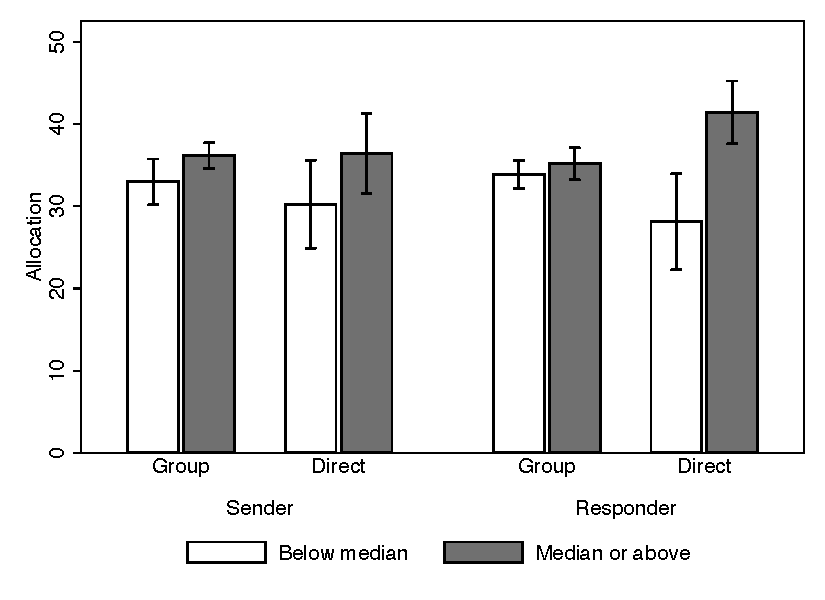
\includegraphics[width=\figwidth]{Reciprocity.pdf}
\end{center}
\end{figure}

\section{Discussion}
\label{sec:conclusion}

Our results suggest that upstream reciprocity is moderated by social boundaries. We distinguish between two types of reciprocity: reciprocated actions and reciprocated intentions \citep{stanca2009testing}.

% Us and Them: we extend to Them and Them
% Intentions generalize, actions don't
% Possible evolutionary channels


\newpage
\printbibliography
%\bibliographystyle{dcu}
%\bibliography{grouprec}

\end{document}
